\documentclass[letterpaper,twocolumn,10pt]{article}
\usepackage{usenix-2020-09}

% to be able to draw some self-contained figs
\usepackage{tikz}
\usepackage{amsmath}

% inlined bib file
\usepackage{filecontents}

%-------------------------------------------------------------------------------
\begin{document}
%-------------------------------------------------------------------------------

%don't want date printed
\date{}

% make title bold and 14 pt font (Latex default is non-bold, 16 pt)
\title{\Large \bf Implementing a Secure Microservice Architecture:\\
  NGINX \& Kubernetes Deployment}

%for single author (just remove % characters)
\author{
{\rm Orchestration: Alexander Moomaw}\\
Eastern Washington University
\and
{\rm Services: Andre Ramirez}\\
Eastern Washington University
\and
{\rm Logging: Brendan Hopkins}\\
Eastern Washington University
\and
{\rm Services: Beighlor Martinez}\\
Eastern Washington University
\and
{\rm Defense: Cameron Olivier}\\
Eastern Washington University
\and
{\rm Frontend: Dillon Pikulik}\\
Eastern Washington University
\and
{\rm Project Management: Chelsea Edwards}\\
Eastern Washington University
}
% copy the following lines to add more authors
% \and
% {\rm Name}\\
%Name Institution
 % end author

\maketitle
%-------------------------------------------------------------------------------
\begin{abstract}
%-------------------------------------------------------------------------------
This paper presents a secure and scalable deployment architecture for web server environments using Kubernetes. 
The deployment incorporates a proxy and web application firewall for enhanced security and modular design. 
Additionally, we introduce our solution to logging and IP banning mechanisms to monitor and restrict unauthorized access. 
Our approach ensures high availability, load balancing, and robust defense against threats, offering a comprehensive framework for modern web applications.
\end{abstract}

%-------------------------------------------------------------------------------
\section{Introduction}
%-------------------------------------------------------------------------------
Ensuring the security and scalability of web server environments is a challenge in modern digital infrastructure. 
As cyber threats become more advanced, it's crucial to implement solutions that protect against unauthorized access 
while also maintaining high availability and performance. 

To address these challenges, we propose a comprehensive deployment architecture by first utilizing Kubernetes, an open-source platform designed for automating deployment, scaling, 
and management of containerized applications. With this platform, we ensure high-availability to prospective users and a modular
environment to build and scale upon as we please. 

To enhance our microservice architecture, we introduced an additional abstraction layer using an NGINX proxy hosted locally on the server. 
This proxy server fetches content from our Kubernetes load balancer, serving as a gateway between our internal services and external communications. 
To mitigate potential threats, we integrated ModSecurity, a well-known web application firewall (WAF), into our proxy. 
ModSecurity monitors and blocks common exploitation methods by referencing a comprehensive rule list that addresses the OWASP Top Ten vulnerabilities.

We realize that exploiting our endpoint services isn't the only attack vector within our environment. 
To address this, we implemented host-level logging to monitor network traffic and identify IP addresses not communicating via SSH or HTTP. 
Additionally, we applied an automated process to block malicious IP addresses, enhancing our overall security posture.



%-------------------------------------------------------------------------------
\section{Orchestration}
%-------------------------------------------------------------------------------
The ultimate challenge of any deployment life cycle is tying all ideas into a single, nicely wrapped package. This is the goal of orchestration.
To implement, or \textit{orchestrate} a deployment such as this, we designed a multi-tiered architectural diagram (Figure~\ref{fig:architecture})
that outlines how every building block in our environment fits together to form a finalized representation of a working project. 

% Add the figure
\begin{figure}[h]
    \centering
    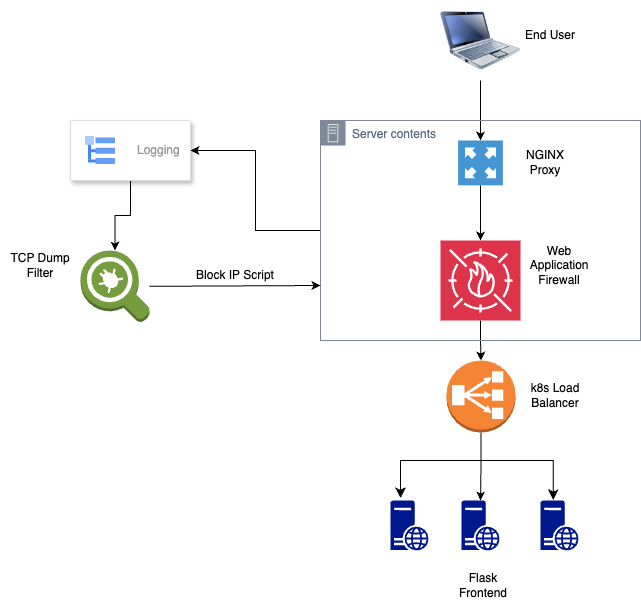
\includegraphics[width=\columnwidth]{resources/diagram.png} 
    \caption{Multi-tiered architectural diagram.}
    \label{fig:architecture}
\end{figure}

To host our content, we utilized Kubernetes. This method first involved integrating a docker image that was specifically designed to host content created by our frontend developers. We then created service and deployment YAML files to control multiple containers behind a load balancer. 

Once we had a functional cluster of orchestrated containers, the next goal was to make our load balancer not the first point of contact between external users and our internal environment. 
This involved integrating an NGINX reverse proxy ~\cite{nginx} on our host machine to facilitate communication without exposing our services directly to the internet. 

To setup an NGINX reverse proxy, we had to install the service then modify the global configuration file in the \texttt{/etc/nginx/conf.d/} directory to specifically mediate communications between external users and our internal load balancer ~\cite{hostinger_nginx_proxy}. The specifics for this step is
very convoluted, essentially we had to define server and location blocks with a \texttt{proxy pass} flag to enable the proxy feature of NGINX.

To tie our scalable, secure environment together on the orchestration end, we installed a web application firewall (WAF) on our reverse proxy to inspect requests being sent to the load balancer ~\cite{linode_modsecurity}. The requests
will be meticulously cross-referenced against a series of rule lists specifically designed to catch exploits matching the OWASP Top Ten vulnerabilities. If a exploit request is detected, the WAF will drop the request and return
a HTTP 403 status code to the threat actor.


%-------------------------------------------------------------------------------
\section{Floating Figures and Lists}

\section{Frontend}
Our Website is called ‘Weather and Jokes’, and includes four pages: 'Home', 'Contact', 'FTP Manual', and 'Login'. The Home page runs two services, ‘Get a Joke’ and ‘Weather Checking’. The Contact page lists each of our team members and their roles within the group. The FTP Manual page gives instructions to our team members on how to use FTP. The FTP Manual page is meant to be a distraction for threat actors and is not fundamental to the actual Website, but rather a ploy to try and catch attackers attempting to use FTP. The final page, Login, takes in user input and redirects back to the log-in page. The log-in page never actually connects to any backend service, this page is used to try and catch potential threat actors attempting to use attacks such as SQL Injections.

%-------------------------------------------------------------------------------
%-------------------------------------------------------------------------------
\section{Logging and IP Gathering}
To enhance security and manage unauthorized access, our deployment includes a mechanism for 
gathering and logging IP addresses. This mechanism is implemented through a series of scripts 
and cron jobs designed to capture IP addresses attempting to access our server on ports other 
than 22 (SSH) and 80 (HTTP), and to log network traffic for further analysis.
In addition to capturing suspicious IP addresses, an hourly logging mechanism is implemented to 
record all network traffic excluding ports 22 and 80. This logging allows for detailed 
analysis of traffic patterns and potential threats. The logs are timestamped and stored systematically
for easy retrieval and review.
The 'Weather and Jokes' web application employs Kubernetes and NGINX within its architecture to provide defenses against several cybersecurity threats. 
We are specifically defending against unauthorized access, SQL injections, Cross-Site Scripting (XSS), session hijacking, and Denial of Service (DoS) attacks. 
In contemplating the perceived capabilities of potential attackers, we recognize that they are likely to possess a high degree of technical sophistication, equipped with the skills necessary to exploit vulnerabilities typical of web applications. 
These attackers might use reconnaissance tools to gain information, and advanced techniques for SQL injections, craft XSS attacks, and leverage automated tools to execute DoS attacks.

To counter these threats, our application utilizes a load balancer within the Kubernetes environment to effectively manage traffic volumes that could potentially lead to DoS attacks. 
This load balancer helps distribute incoming traffic evenly across available servers, preventing any single server from becoming overwhelmed. We sanitize user input, protecting against XSS, and logging the attempts they made so we understand more of our attackers attacks and motives.
Additionally, NGINX, configured as a reverse proxy, is important in safeguarding against unauthorized access and filtering out malicious requests. It acts as a gatekeeper, routing all incoming traffic through its server and using ModSecurity-a web application firewall(Talked more about later)—to identify and block threats identified from patterns typical in SQL injections and XSS. 
Moreover, NGINX enhances the security of user sessions by managing encrypted connections, a crucial feature for preventing session hijacking. 
These encrypted channels ensure that session tokens, critical for maintaining user session integrity, are not intercepted or tampered with by unauthorized parties.
Through the strategic implementation of Kubernetes and NGINX, our application is well-prepared to defend against a wide spectrum of cybersecurity threats.

%-------------------------------------------------------------------------------

%-------------------------------------------------------------------------------
\section{Floating Figures and Lists}

Here you may want your evaluation methodology...

\label{sec:figs}
%-------------------------------------------------------------------------------


%---------------------------
\begin{figure}
\begin{center}
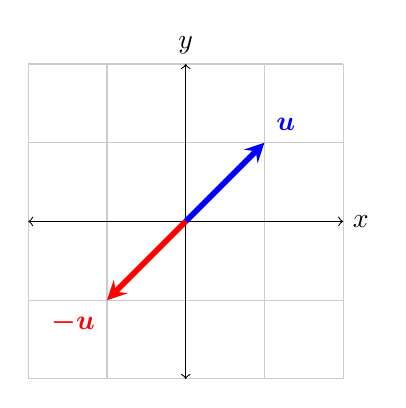
\begin{tikzpicture}
  \draw[thin,gray!40] (-2,-2) grid (2,2);
  \draw[<->] (-2,0)--(2,0) node[right]{$x$};
  \draw[<->] (0,-2)--(0,2) node[above]{$y$};
  \draw[line width=2pt,blue,-stealth](0,0)--(1,1)
        node[anchor=south west]{$\boldsymbol{u}$};
  \draw[line width=2pt,red,-stealth](0,0)--(-1,-1)
        node[anchor=north east]{$\boldsymbol{-u}$};
\end{tikzpicture}
\end{center}
\caption{\label{fig:vectors} Text size inside figure should be as big as
  caption's text. Text size inside figure should be as big as
  caption's text. Text size inside figure should be as big as
  caption's text. Text size inside figure should be as big as
  caption's text. Text size inside figure should be as big as
  caption's text. }
\end{figure}
%% %---------------------------


Here's a typical reference to a floating figure:
Figure~\ref{fig:vectors}. Floats should usually be placed where latex
wants then. Figure\ref{fig:vectors} is centered, and has a caption
that instructs you to make sure that the size of the text within the
figures that you use is as big as (or bigger than) the size of the
text in the caption of the figures. Please do. Really.

In our case, we've explicitly drawn the figure inlined in latex, to
allow this tex file to cleanly compile. But usually, your figures will
reside in some file.pdf, and you'd include them in your document
with, say, \textbackslash{}includegraphics.

Lists are sometimes quite handy. If you want to itemize things, feel
free:

\begin{description}
  
\item[fread] a function that reads from a \texttt{stream} into the
  array \texttt{ptr} at most \texttt{nobj} objects of size
  \texttt{size}, returning returns the number of objects read.

\item[Fred] a person's name, e.g., there once was a dude named Fred
  who separated usenix.sty from this file to allow for easy
  inclusion.
\end{description}

\noindent
The noindent at the start of this paragraph in its tex version makes
it clear that it's a continuation of the preceding paragraph, as
opposed to a new paragraph in its own right.


\subsection{LaTeX-ing Your TeX File}
%-----------------------------------

People often use \texttt{pdflatex} these days for creating pdf-s from
tex files via the shell. And \texttt{bibtex}, of course. Works for us.


%-------------------------------------------------------------------------------
\bibliographystyle{plain}
\bibliography{refs}

%%%%%%%%%%%%%%%%%%%%%%%%%%%%%%%%%%%%%%%%%%%%%%%%%%%%%%%%%%%%%%%%%%%%%%%%%%%%%%%%
\end{document}
%%%%%%%%%%%%%%%%%%%%%%%%%%%%%%%%%%%%%%%%%%%%%%%%%%%%%%%%%%%%%%%%%%%%%%%%%%%%%%%%

%%  LocalWords:  endnotes includegraphics fread ptr nobj noindent
%%  LocalWords:  pdflatex acks
